% Gemini theme
% https://github.com/anishathalye/gemini
%
% We try to keep this Overleaf template in sync with the canonical source on
% GitHub, but it's recommended that you obtain the template directly from
% GitHub to ensure that you are using the latest version.

\documentclass[final]{beamer}

% ====================
% Packages
% ====================

\usepackage[T1]{fontenc}
\usepackage{lmodern}
\usepackage[size=custom,width=120,height=72,scale=1.0]{beamerposter}
\usetheme{gemini}
\usecolortheme{gemini}
\usepackage{graphicx}
\usepackage{booktabs}
\usepackage{tikz}
\usepackage[font=small,skip=1pt]{caption}
\usepackage{pgfplots}

\usepackage{colortbl}

\usepackage{xcolor}
\usepackage{pifont}

\newcommand{\xmark}{\ding{55}}%
\newcommand{\CheckmarkBold}{\ding{51}}%

% ====================
% Lengths
% ====================

% If you have N columns, choose \sepwidth and \colwidth such that
% (N+1)*\sepwidth + N*\colwidth = \paperwidth
\newlength{\sepwidth}
\newlength{\colwidth}
\setlength{\sepwidth}{0.025\paperwidth}
\setlength{\colwidth}{0.3\paperwidth}

\newcommand{\separatorcolumn}{\begin{column}{\sepwidth}\end{column}}

% ====================
% Title
% ====================

\addtobeamertemplate{headline}{} 
{
\begin{tikzpicture}[remember picture,overlay] 
\node [shift={(-4 cm,-4cm)}] at (current page.north east) {
\includegraphics[height=5cm]{figs/FSU_Seal.png}}; 
\end{tikzpicture} 
}

\addtobeamertemplate{headline}{} 
{
\begin{tikzpicture}[remember picture,overlay] 
\node [shift={(4 cm,-4cm)}] at (current page.north west) {
\includegraphics[height=5cm]{figs/FSU_Seal.png}}; 
\end{tikzpicture} 
}


\title{
  {Analyzing Hardware Parameters in GPU based HPC Platform}}

\author{Saptarshi Bhowmik\textsuperscript{1}, Nikhil Jain\textsuperscript{2},, Abhinav Bhatele\textsuperscript{3} and Xin Yuan\textsuperscript{1}} % Author(s)

\institute{1. Florida State University, 2. NVIDIA, Inc, 3. University of Maryland}

% ====================
% Body
% ====================

\begin{document}

\begin{frame}[t]
\begin{columns}[t]
\separatorcolumn

\begin{column}{0.2\textwidth}

\begin{alertblock}{Goals}
    \begin{itemize}
        \item \textbf{ Analyze if a HPC system with fewer nodes each with more compute capability perform better than a system with more nodes each with lesser compute capability.}
        \item \textbf{ Use discrete-event simulations to study several parameters including network bandwidth, number of GPUs per node  in the context of two most popular network topology Fat-Tree and  1D-Dragonfly.}
    \end{itemize}
\end{alertblock}



  \begin{block}{Introduction}
    Today's high-end HPC clusters employ many GPUs per node. The performance of applications on such a platform depends heavily on the interconnection network performance [1]. As such, it is important to understand the impact of hardware parameters on the overall application and system performance. In this research, we perform extensive simulation study to understand hardware parameters and their impact on the performance of HPC workload.
    
% \begin{figure}
% \centering
% \centering
% 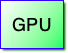
\includegraphics[width=3cm, height=3cm]{figs/1gpu.png}
% \captionsetup{labelformat=empty}
% \caption{Ratio of Bandwidth,GPUs per node mapping for Stencil in Fat-Tree}
% \end{figure}
    
  \end{block}

  \begin{block}{Method}
  
    \begin{itemize}
    
        \heading{Tracer-CODES}
        We use the discrete event driven simulator, TraceR-CODES\cite{b4} to replay the application traces. The simulator network model is used to implement the interconnect topology, on top of which the traces are replayed.
        \newline
        \newline
        \newline
            \begin{figure}[H]
            \centering
            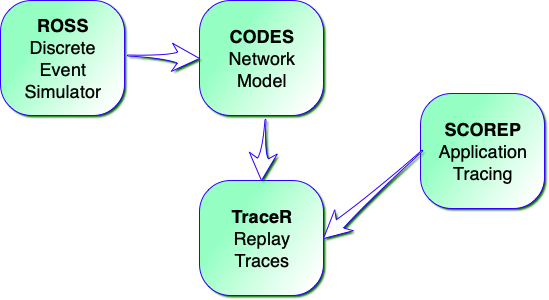
\includegraphics[width=18cm, height=11.25cm]{figs/Tracer.png}
            \caption{TraceR-CODES workflow}
            \end{figure}
        \vspace{-1cm}
         \heading{Applications}
        
        Six popular HPC Applications are use in the simulation.
        \begin{table}
        % \begin{adjustbox}{width=18cm,height=11.25cm}
        
        \begin{tabular}{|c|c|c|} \hline
        \hline
        \textbf{Traces} & \textbf{Computation Intensive} & \textbf{Communication Intensive} \\ \hline
        \cellcolor{Blue!10}Stencil4d & \cellcolor{Blue!10}\xmark & \cellcolor{Blue!10}\CheckmarkBold  \\    \hline
        Kripke & \CheckmarkBold & \xmark  \\    \hline
        \cellcolor{Blue!10}Laghos & \cellcolor{Blue!10}\CheckmarkBold & \cellcolor{Blue!10}\xmark  \\    \hline
        Subcomm-a2a & \xmark & \CheckmarkBold  \\    \hline
        \cellcolor{Blue!10}Sw4lite & \cellcolor{Blue!10}\CheckmarkBold  & \cellcolor{Blue!10}\CheckmarkBold  \\    \hline
        Amg & \CheckmarkBold  & \CheckmarkBold  \\    \hline
        \end{tabular}
        % \end{adjustbox}


\caption{Profiles of Application Traces}
\end{table}
        
        
    \end{itemize}



  \end{block}

\end{column}

\separatorcolumn

\begin{column}{0.5\textwidth}




  \begin{block}{Simulation Environment Parameters}
  \begin{column}{0.3\textwidth}
  \heading{Network Topologies}

  \begin{figure}
\centering
\begin{minipage}[t][2cm][t]{.40\textwidth}
\centering
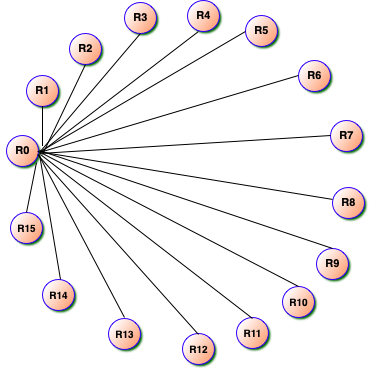
\includegraphics[width=\linewidth]{figs/1Dgroup.png}
% \captionsetup{labelformat=empty}
\caption{1D-Dragonfly Group}
\label{fig:13a}
\end{minipage}
\separatorcolumn
\begin{minipage}[t][2cm][t]{.40\textwidth}
\centering
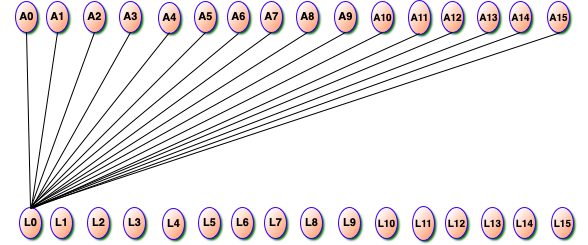
\includegraphics[width=1\linewidth,height=5cm]{figs/fat-tree.png}
% \captionsetup{labelformat=empty}
\caption{Fat-Tree Pod}
\label{fig:13b}
\end{minipage}
%\caption{}
\end{figure}



\begin{table}

        \begin{tabular}{|c|c|c|c|c} \hline
        \hline
        \textbf{Topology} & \textbf{1-GPU/Node} & \textbf{2-GPU/Node} & \textbf{4-GPU/Node} & \textbf{8-GPU/Node}  \\ \hline
        \cellcolor{Blue!10}1D-Dragonfly & \cellcolor{Blue!10}16 Group & 
        \cellcolor{Blue!10}8 Group & 
        \cellcolor{Blue!10}4 Group & 
        \cellcolor{Blue!10}2 Group  \\    \hline
        
        \cellcolor{Blue!10}Fat-Tree & \cellcolor{Blue!10}8 Pods & 
        \cellcolor{Blue!10}8 Pods & 
        \cellcolor{Blue!10}4 Pods & 
        \cellcolor{Blue!10}2 Pods  \\    \hline
       
        \end{tabular}
        % \end{adjustbox}


\caption{Profiles of Application Traces}
\end{table}



  
  \end{column}
  \begin{column}{0.3\textwidth}
  \heading{Bandwidth}
  \newline
  \newline
  \newline
  \newline
  \textbf{Default Setting : }
  \newline
  Link Bandwidth = 11.9 Gb/s
  \newline
  Internal Bandwidth = 11.9 Gb/s
  \newline
  \newline
  We use 8 more bandwidth, x/16, x/8, x/4, x/2, 2x, 4x, 8x, 16x, for our simulations.
  \end{column}
  \begin{column}{0.3\textwidth}
  \heading{GPUs per node}
  
  \begin{figure}
\centering
\begin{minipage}[t][2cm][t]{.40\textwidth}
\centering
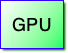
\includegraphics[width=0.25\linewidth]{figs/1gpu.png}
% \captionsetup{labelformat=empty}
\caption{1-GPU/Node}
\label{fig:13a}
\end{minipage}
\separatorcolumn
\begin{minipage}[t][2cm][t]{.40\textwidth}
\centering
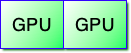
\includegraphics[width=0.5\linewidth]{figs/2gpu.png}
% \captionsetup{labelformat=empty}
\caption{2-GPU/Node}
\label{fig:13b}
\end{minipage}
%\caption{}
\end{figure}
\vspace{2cm}
\begin{figure}
\centering
\begin{minipage}[t][2cm][t]{.40\textwidth}
\centering
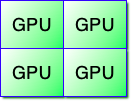
\includegraphics[width=0.5\linewidth]{figs/4gpu.png}
% \captionsetup{labelformat=empty}
\caption{4-GPU/Node}
\label{fig:13a}
\end{minipage}
\separatorcolumn
\begin{minipage}[t][2cm][t]{.40\textwidth}
\centering
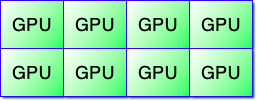
\includegraphics[width=1\linewidth]{figs/8gpu.png}
% \captionsetup{labelformat=empty}
\caption{8-GPU/Node}
\label{fig:13b}
\end{minipage}
%\caption{}
\end{figure}

\vspace{2cm}
From 1-GPU/Node, 2-GPU/Node, 4-GPU/Node and 8-GPU/Node configuration.

  \end{column}

  \end{block}


\vspace{-2cm}

  \begin{block}{Result}
  \heading{Impact of GPUs per Node}
 \begin{figure}
\centering
\begin{minipage}[t][2cm][t]{.45\textwidth}
\centering
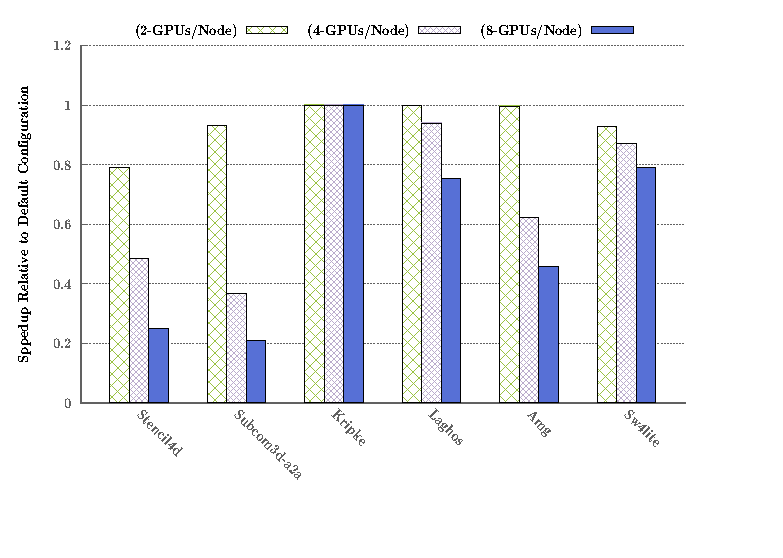
\includegraphics[width=1\linewidth,height=12cm]{figs/ftree-x-mapping-all.eps}
% \captionsetup{labelformat=empty}
\caption{Fat-Tree}
\label{fig:13a}
\end{minipage}
\separatorcolumn
\begin{minipage}[t][2cm][t]{.45\textwidth}
\centering
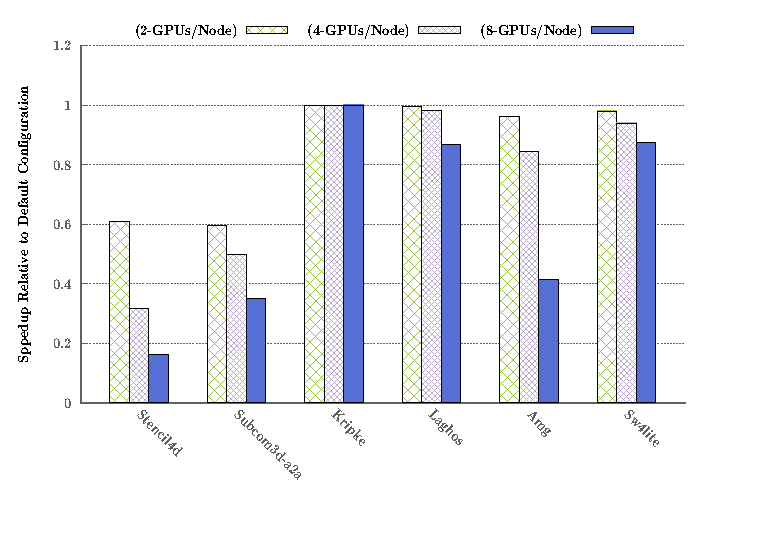
\includegraphics[width=1\linewidth,height=12cm]{figs/dfly-x-mapping-all.eps}
% \captionsetup{labelformat=empty}
\caption{1D-Dragonfly}
\label{fig:13b}
\end{minipage}
%\caption{}
\end{figure}
Communication intensive applications experience more slowdown than applications with computation.
 \vspace{-1cm}

\heading{Impact of Bandwidth}
 \begin{figure}
\centering
\begin{minipage}[t][2cm][t]{.45\textwidth}
\centering
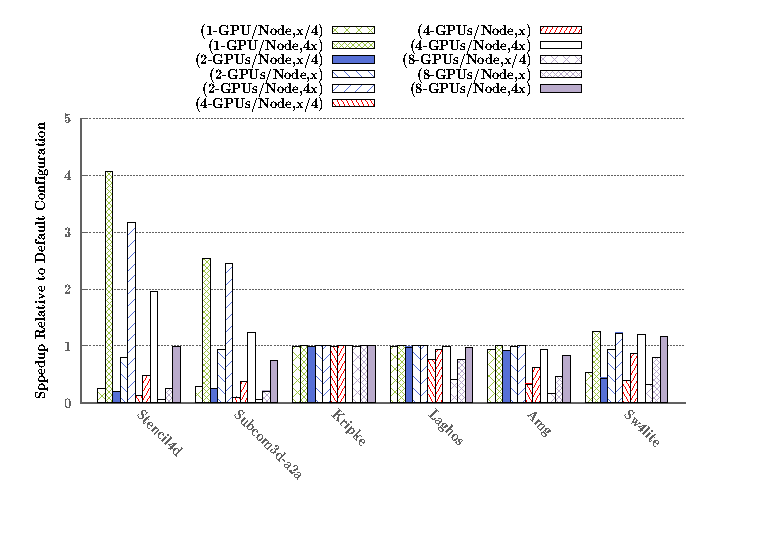
\includegraphics[width=1\linewidth]{figs/ftree-bw-mapping-all.eps}
\caption{Fat-Tree}
\label{fig:13a}
\end{minipage}
\separatorcolumn
\begin{minipage}[t][2cm][t]{.45\textwidth}
\centering
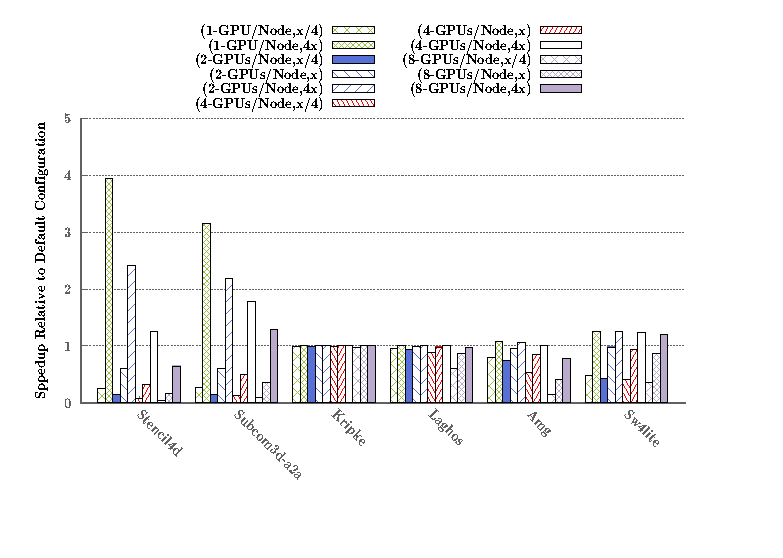
\includegraphics[width=1\linewidth]{figs/dfly-bw-mapping-all.eps}
% \captionsetup{labelformat=empty}
\caption{1D-Dragonfly}
\label{fig:13b}
\end{minipage}
% \captionsetup{labelformat=empty}
%\caption{1d-Dragonfly Topology}
\end{figure}
Applications performance speedup when the bandwidth is increased.
\newline
The increase is more pronounced is full computational intensive applications.

  \end{block}


\end{column}

\separatorcolumn

\begin{column}{0.2\textwidth}

  \begin{block}{Conclusion}

    \begin{itemize}
        \item As the number of GPU per node increases, the node becomes more intensive, and thus, there is a slowdown in application performance as the communication/computation capacity of the network reduces.
        \item As the number of GPU per node increases, more bandwidth is needed to substantiate the slowdown in application performance.
        \item Every application has a sweet spot where it is performing the best.
    \end{itemize}

  \end{block}

  \begin{block}{Future Works}

    \begin{itemize}
        \item Study how other simulation environment and hardware design, such as NIC scheduling policies effect the performance of applications
    
        \item Profile more HPC applications and find the performance of those applications across the currently deployed GPU based interconnect topology,
    \end{itemize}
    

  \end{block}

  \begin{block}{References}

    \begin{thebibliography}{00}
    \bibitem{b1} Jain, N., Bhatele, A., Howell, L. H., Böhme, D., Karlin, I., León, E. A., ... & Leininger, M. L. (2017, November). Predicting the performance impact of different fat-tree configurations. In Proceedings of the International Conference for High Performance Computing, Networking, Storage and Analysis (pp. 1-13).
    \bibitem{b2} Kim, J., Dally, W. J., Scott, S., & Abts, D. (2008, June). Technology-driven, highly-scalable dragonfly topology. In 2008 International Symposium on Computer Architecture (pp. 77-88). IEEE.
    \bibitem{b3} Knüpfer, A., Rössel, C., an Mey, D., Biersdorff, S., Diethelm, K., Eschweiler, D., ... & Nagel, W. E. (2012). Score-p: A joint performance measurement run-time infrastructure for periscope, scalasca, tau, and vampir. In Tools for High Performance Computing 2011 (pp. 79-91). Springer, Berlin, Heidelberg.
    \bibitem{b4} Acun, B., Jain, N., Bhatele, A., Mubarak, M., Carothers, C. D., & Kale, L. V. (2015, August). Preliminary evaluation of a parallel trace replay tool for hpc network simulations. In European Conference on Parallel Processing (pp. 417-429). Springer, Cham.
    \bibitem{b5} Alzaid, Z. S. A., Bhowmik, S., Yuan, X., & Lang, M. (2020, June). Global link arrangement for practical Dragonfly. In Proceedings of the 34th ACM International Conference on Supercomputing (pp. 1-11). Magnetics Japan, p. 301, 1982].


    \end{thebibliography}

  \end{block}

\end{column}

\separatorcolumn
\end{columns}
\end{frame}

\end{document}
